\chapter{Nonlinear filtering} \label{chap:kalman}
Nonlinearity is a common phenomenon in reality. Real world consists of various nonlinear systems. Practical situations (such as defining underwater vehicle location) often demand dealing with nonlinear systems by using approximations that eventually lead to linearity or some other tricks. The solution obtained this way is claimed to be sub-optimal - not perfectly tuned, but indeed useful. The problem is to consecutively make an estimation of the state of a dynamic system using a sequence of noisy measurements \cite{ristic04}. State-space approach turns out to be suitable choice when dealing with both nonlinearity and sort of estimation (filtering) where the whole procedure involves more than one variable. Number of filters have been designed to deal with the phenomenon. Depending on how they handle nonlinearity, they could be roughly categorized as \cite{ristic04}: 
\begin{itemize}
\item those that use analytic approximations (e.g. EKF)
\item those that use numerical approximations
\item those that use multiple models
\item those that use sampling (e.g. UKF)
\end{itemize} 
Since approximations lead to eventual transformation into linear system, a short overview of linear Kalman Filter (KF) is given in order to make an introduction on something that will be the basis for methods presented.
%%%%%%%%%%%%%%%%%%%%%%%%%%%%%%%%%%%%%%%%%%%%
\section{Kalman Filter (KF)}  \label{sec:kf}
KF \cite{kalman60}  is a well known mathematical tool that offers solution to \textit{linear-quadratic problem} in form of estimator \cite{grewal01,ristic04}. Such linear estimator is optimal in terms of any quadratic function of estimation error \cite{grewal01}. It is based on an iterative and recursive process, well suited framework for blending together different sensor measurements. Mathematically speaking - world consists of variety of systems that change their state $(\vect{x}(k))$ in time. Guided by this foundation, science has established concept of \textit{linear dynamic system model} (Table ~\ref{tab:system}) consisted of \textit{process model} and \textit{measurement model}. \textit{Process model} (Table ~\ref{tab:system}) is perturbed by Gaussian white noise $(\vect{n})$. It emulates the behaviour of a phenomenon (change of the states) together with its hereditary randomness. \textit{Measurement model} (Table ~\ref{tab:system}) emulates observations of the system state. Observations are expressed as linear functions of state variables corrupted with Gaussian white measurement noise $(\vect{m})$, similarly as the process model itself. System can receive control inputs $(\vect{u}(k))$. Covariances of process and measurement Gaussian white noises, $\vect{Q}$ and $\vect{R}$ respectfully, are important components of filtering algorithm ~\ref{alg:kf}.
\begin{table*}
\centering
	\caption{Overview of the state-system models.}
	\label{tab:system}
\begin{tabular}{cc}
\toprule
\multicolumn{2}{c}{System models overview} \\
\multicolumn{2}{c}{$\vect{x}$ - system state vector, $\vect{u}$ - control input, $\vect{n}$ - process noise, $\vect{m}$ - measurement noise} \\
\midrule
\multirow{1}{*}{Linear System Model}  &  \multirow{1}{*}{Nonlinear System Model} \\
\multicolumn{2}{c}{process model:} \\
\multirow{2}{*}{$\vect{x}(k) = \vect{A}\vect{x}(k-1)+\vect{B}\vect{u}(k)+\vect{n}(k-1)$} 
									& \multirow{2}{*}{$\vect{x}(k) = f(\vect{x}(k-1),\vect{u}(k),\vect{n}(k-1))$} \\ \\
\multicolumn{2}{c}{measurement model:} \\
\multirow{2}{*}{$\vect{z}(k) = \vect{H}\vect{x}(k)+\vect{m}(k)$} 
									& \multirow{2}{*}{$\vect{z}(k) = h(\vect{x}(k),\vect{m}(k))$} \\ \\
\bottomrule
$\vect{A}$ matrix associates $(\vect{x}(k-1))$ and $(\vect{x}(k))$ & $f()$ nonlinear process function \\
$\vect{B}$ matrix associates $(\vect{u}(k-1))$ and $(\vect{x}(k))$ & $h()$ nonlinear measurement function \\
$\vect{H}$ matrix associates $(\vect{x}(k))$   and $(\vect{z}(k))$ &   \\
\\
\multicolumn{2}{c}{$E\lbrace \vect{n}(k) \rbrace = E\lbrace \vect{m}(k) \rbrace = 0$} \\ 
\multicolumn{2}{c}{$E\lbrace \vect{n}(k) \vect{n}(j)^{T} \rbrace =  \delta_{kj} \vect{Q}, E\lbrace \vect{m}(k) \vect{m}(j)^{T} \rbrace = \delta_{kj} \vect{R}$} 
\end{tabular} 
\end{table*}

The Discrete Kalman Filter is an optimal unbiased minimum mean squared error estimator. It is a calculation process that works recursively, passing iterations as shown in diagram ~\ref{fig:diagram-kalman}. Kalman filter uses three basic steps: prediction, measurement and update. One iteration uses process equation, next one proceeds further using prediction result within the observation equation. Recursion continues each time referring to previous filter output.

Assumptions that KF uses:
\begin{itemize}
\item distribution of a random variable is assumed to be Gaussian, therefore mean and variance can fully describe it
\item linear transform of a Gaussian distribution gives another Gaussian distribution 
\end{itemize}
In spirit of that, noise vectors ($\vect{n}, \vect{m}$)  and thus linearly derived state and observation vectors ($\vect{x}, \vect{z}$) are Gaussian. Another assumption is that noise vectors $n$, $m$ have zero mean values (``white Gaussian'') and that their elements are not correlated, resulting in diagonal matrices $\vect{Q}$ and $\vect{R}$ (Table ~\ref{tab:system}).

\begin{wrapfigure}{r}{0.5\textwidth}
\vspace{-10pt}
  \centering
    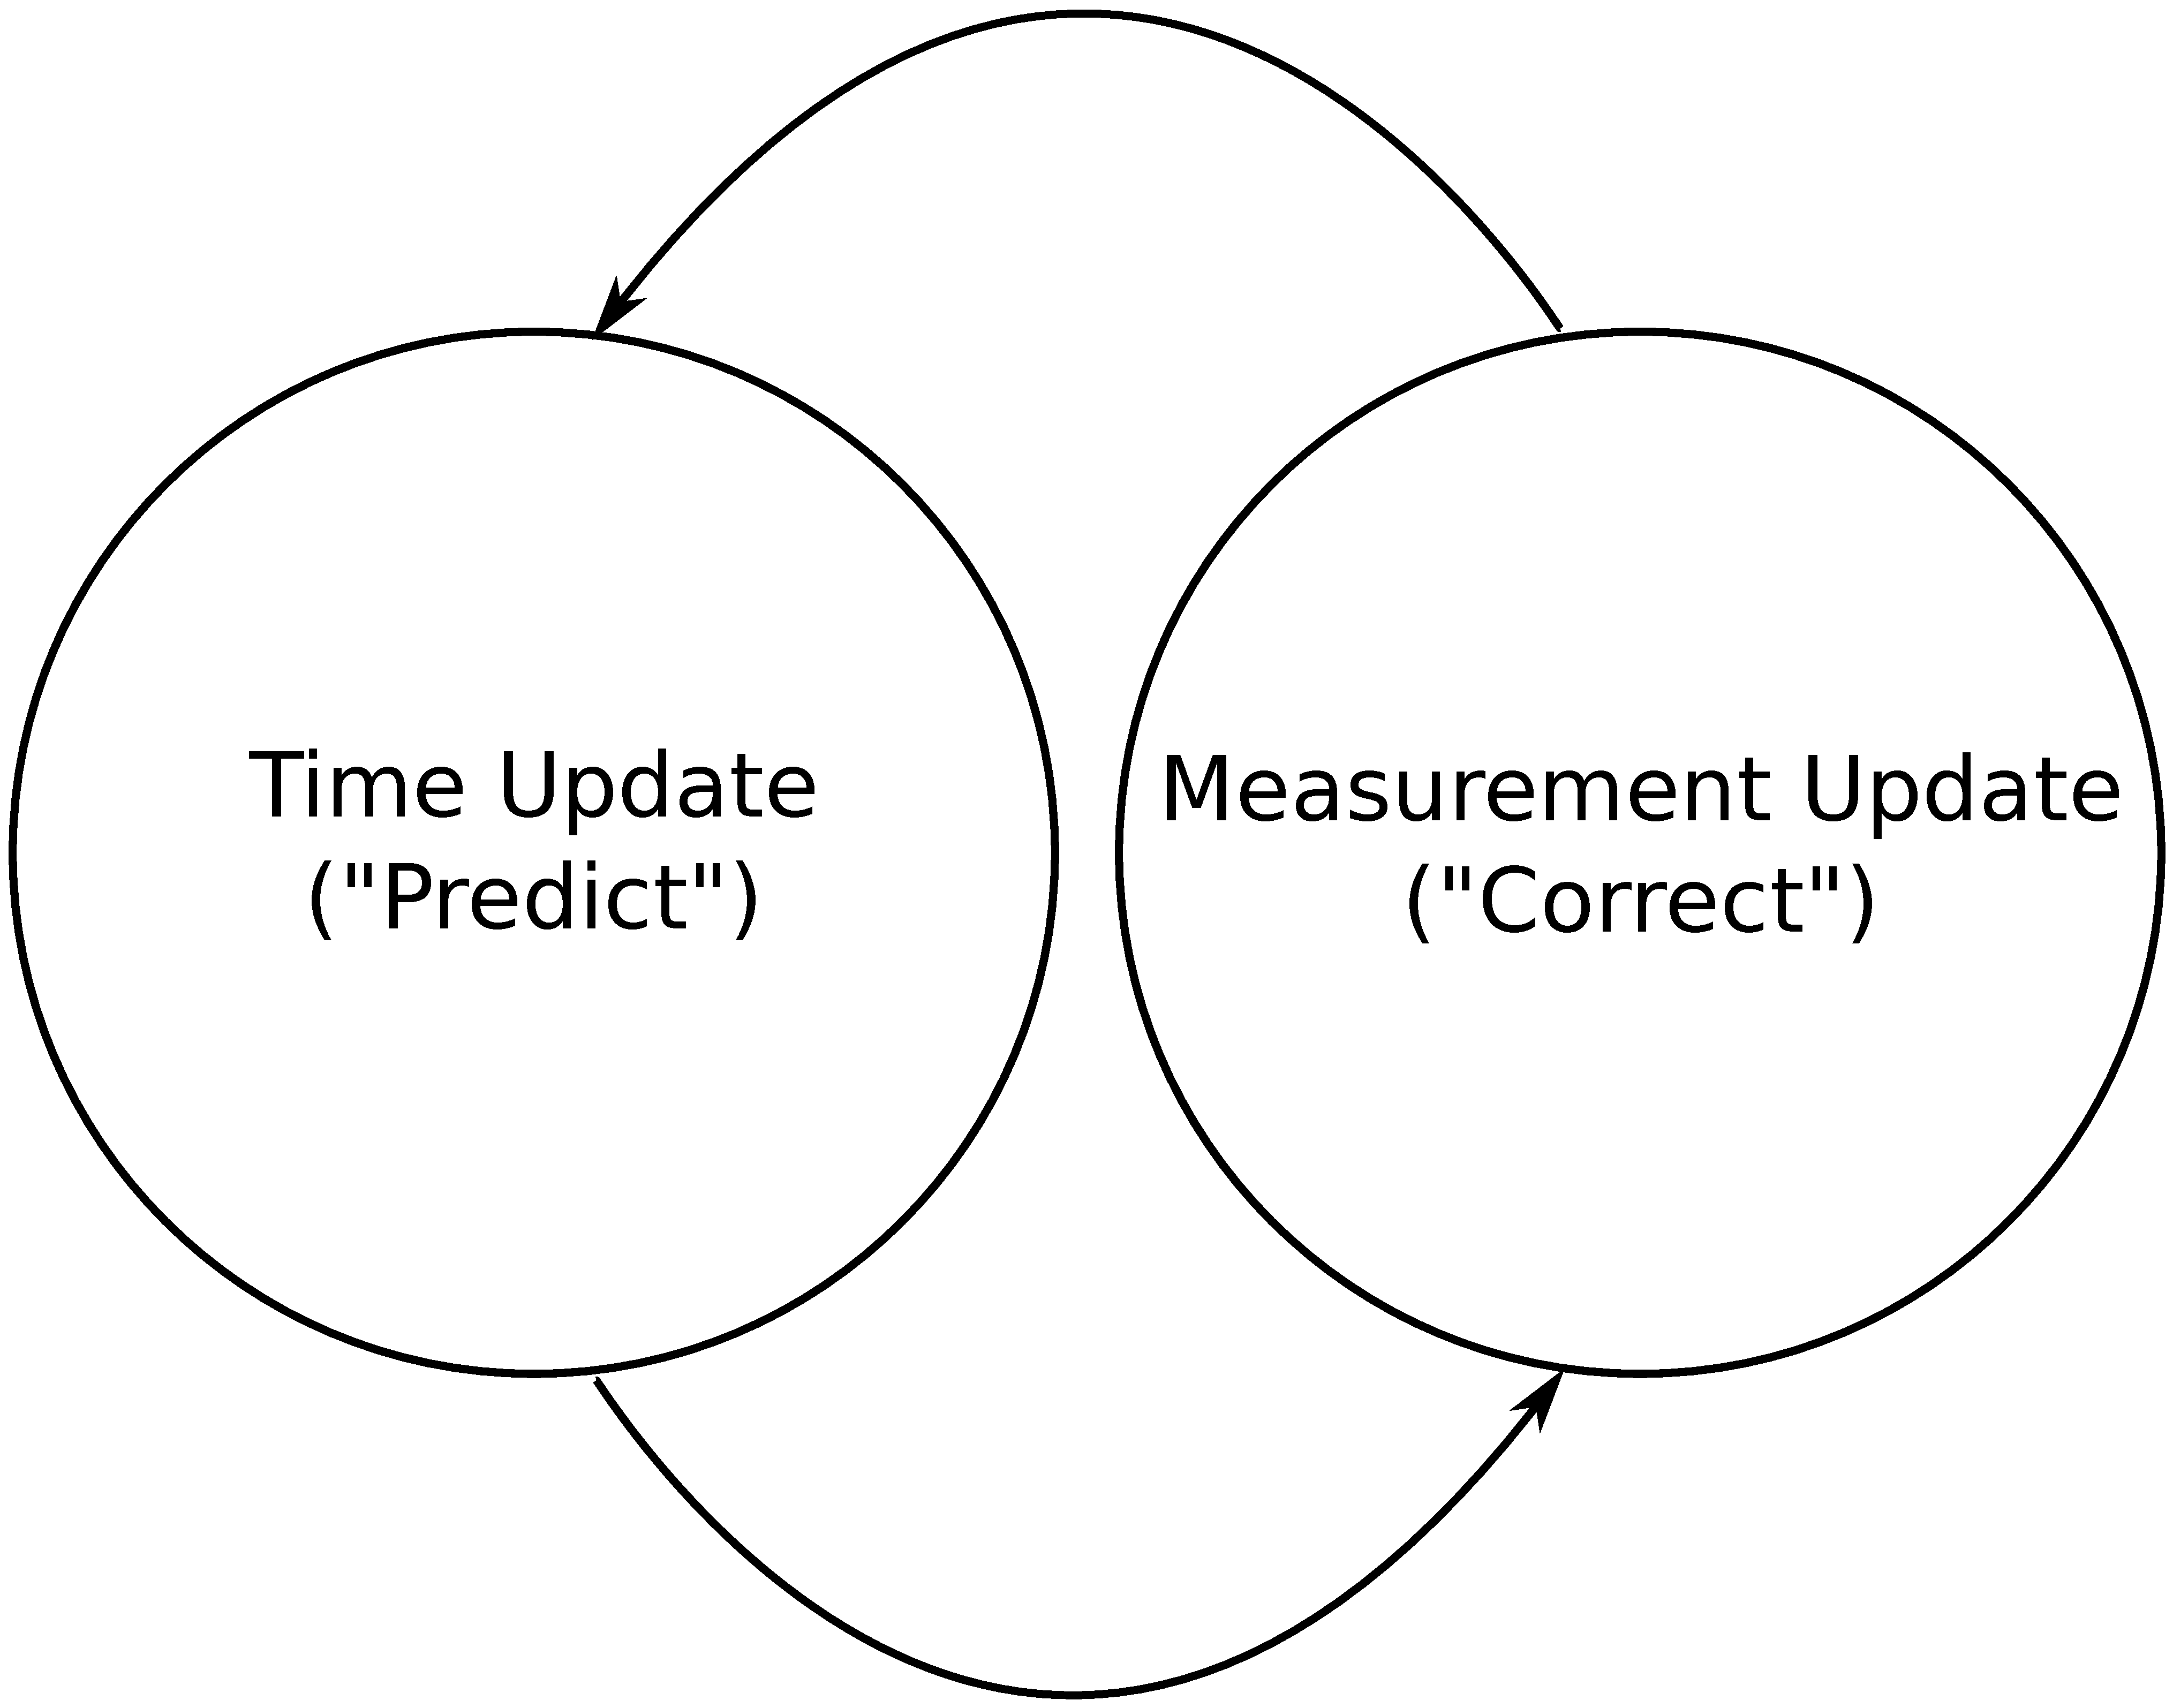
\includegraphics[width=0.4\textwidth]{kalman/fig/diagram-kalman.eps}
  \caption{Filtering process.}
\vspace{-10pt}
\label{fig:diagram-kalman}
\end{wrapfigure}

KF can be summarized with the set of formulas given in Algorithm ~\ref{alg:kf}. The aim of the equations is to recursively obtain the estimate of the state vector ${\vect{\hat{x}}}$ and the uncertainty of such estimate. Uncertainty is described as state variance $\vect{P}(k) = E\lbrace (\vect{x}(k) - \vect{\hat{x}}(k)) (\vect{x}(k) - \vect{\hat{x}}(k))^{T} \rbrace$. KF defines states as having elements with Gaussian distribution, thus mean value is used as an estimate and variance as a measure of how far the values are spread out around mean. Notation is following the one form Table ~\ref{tab:system}. $\vect{\hat{x}}(k \mid l)$ is a state estimate at the time k using observations obtained until time moment $m$. It is a recursive estimator since every estimation relies on previous state estimation and current observation (measurement). Therefore, although history of previous observations is not directly used, it is still incorporated in previous state estimation. Previous state estimation is used in current state estimate due to recursive nature of the algorithm. Uncertainty is updated after each estimate or prediction. I is, depending on case, incorporating the transformation uncertainty $\vect{Q}$ or the noise uncertainty $\vect{R}$. Innovation $\nu$ is difference between observation and predicted observation. Both innovation and its covariance matrix $\vect{S}$ are included in calculation of Kalman gain $K$. Kalman gain does the final state estimate correction ~\ref{alg:kf} influenced by recent observation and makes the uncertainty optimal with respect to quadratic estimation error criteria.
\begin{algorithm}%[h!]
\caption{The Discrete Kalman Filter} \label{alg:kf}
\begin{algorithmic}
\REQUIRE $E\lbrace \vect{x}(0) \rbrace = \vect{x}(0) = \vect{\hat{x}}(0)$
\COMMENT{initialize state}
\REQUIRE $\vect{P}(0) = \delta_{jk} \vect{P_{0}} $ 
\COMMENT {initialize covariance}
\LOOP 
	\STATE $k \Leftarrow k+1$ 
	\STATE $\vect{\hat{x}}(k \mid k-1) = \vect{A} \vect{\hat{x}}(k-1) + \vect{B} \vect{u}(k)$
	\COMMENT {state prediction}
	\STATE $\vect{P}(k \mid k-1) = \vect{A} \vect{P}(k-1) \vect{A}^{T} + \vect{Q}$
	\COMMENT {state prediction uncertainty}	
	
	\STATE $\nu = \vect{z}(k) - \vect{H} \vect{\hat{x}}(k \mid k-1)$	
	\COMMENT {innovation}
	\STATE $\vect{S} = \vect{H} \vect{P}(k \mid k-1) \vect{H}^{T} + \vect{R}$	
	\COMMENT {innovation uncertainty}	
	\STATE $\vect{K} = \vect{P}(k \mid k-1) \vect{H}^{T} \vect{S}^{-1}$	
	\COMMENT {``Kalman gain''}	
	
	\STATE $\vect{\hat{x}}(k) = \vect{\hat{x}}(k \mid k-1) + \vect{K} \nu$
	\COMMENT {state correction} 
	\STATE $\vect{P}(k) = (\vect{I}-\vect{K}\vect{H})\vect{P}(k \mid k-1)$
	\COMMENT {state correction uncertainty}
	\RETURN $\vect{\hat{x}}(k), \vect{P}(k)$
\ENDLOOP
\end{algorithmic}
\end{algorithm}
Although essentially intended for dealing with linear system, KF formulas will be important component of the process of nonlinear filtering accomplished with Extended Kalman Filter (EKF) or Unscented Kalman Filter (UKF). 
%%%%%%%%%%%%%%%%%%%%%%%%%%%%%%%%%%%%%%%%%%%%%%%%   
\section{Extended Kalman Filter} \label{sec:ekf}
Idea is that the system can be described with set of states that evolve in time according to mathematical functions that are nonlinear in many applications. Table ~\ref{tab:system} gives an overview, categorizing systems as linear or nonlinear. Nonlinear state prediction would use previous state estimate and mean value of the process noise:
\begin{equation}
\vect{\hat{x}}(k \mid k-1) = f(\vect{\hat{x}}(k-1), \vect{u}(k), 0)
\label{eq:state-pred-nonlin}
\end{equation} 
EKF is intended for solving sub-optimal state estimation of a nonlinear system. The main characteristic of EKF is that it analytically approximates - linearises - process and measurement functions ($f()$ and $h()$, Table ~\ref{tab:system}). Linearisation implies approximating these functions with their first derivative around current prediction, similarly as the ordinary functions are approximated with Taylor polynomials of first degree. In this case derivation is slightly more complex since model functions $f()$ and $h()$ take several input vectors and output the resulting vector. Hence, derivation will consist of partial derivation of process per state input vector (Equation ~\ref{eq:der-proc-state}) and per noise input vector (Equation ~\ref{eq:der-proc-noise}). And partial derivation of measurement function per state (Equation ~\ref{eq:der-mes-state}) and measurement noise (Equation ~\ref{eq:der-mes-noise}). Partial derivatives themselves will be Jacobian matrices considering that vector is derived per vector. 
\begin{equation}
\vect{F}(k) = \frac{\partial f}{\partial x} (\vect{\hat{x}}(k \mid k-1), \vect{u}(k), 0)
\label{eq:der-proc-state}
\end{equation} 
\begin{equation}
\vect{W}(k) = \frac{\partial f}{\partial n} (\vect{\hat{x}}(k \mid k-1), \vect{u}(k), 0)
\label{eq:der-proc-noise}
\end{equation}
\begin{equation}
\vect{H}(k) = \frac{\partial h}{\partial x} (\vect{\hat{x}}(k \mid k-1), 0)
\label{eq:der-mes-state}
\end{equation} 
\begin{equation}
\vect{V}(k) = \frac{\partial h}{\partial m} (\vect{\hat{x}}(k \mid k-1), 0)
\label{eq:der-mes-noise}
\end{equation}
Subsequently, filtering process can be treated similarly as classic, discrete linear Kalman filter introduced in previous section. 
\begin{algorithm}%[h!]
\caption{The Discrete Extended Kalman Filter} \label{alg:ekf}
\begin{algorithmic}
\REQUIRE $E\lbrace \vect{x}(0) \rbrace = \vect{x}(0) = \vect{\hat{x}}(0)$
\COMMENT{initialize state}
\REQUIRE $\vect{P}(0) = \delta_{jk} \vect{P_{0}} $ 
\COMMENT {initialize covariance}
\LOOP 
	\STATE $k \Leftarrow k+1$ 
	\STATE $\vect{\hat{x}}(k \mid k-1) = f(\vect{\hat{x}}(k-1), \vect{u}(k), 0)$
	\COMMENT {state prediction}
	\STATE $\vect{P}(k \mid k-1) = \vect{F}(k) \vect{P}(k-1) \vect{F}^{T}(k) + \vect{W}(k) \vect{Q} \vect{W}^{T}(k)$
	\COMMENT {state prediction uncertainty}	
	
	\STATE $\nu = \vect{z}(k) - h(\vect{\hat{x}}(k \mid k-1), 0)$	
	\COMMENT {innovation}
	\STATE $\vect{S} = \vect{H}(k) \vect{P}(k \mid k-1) \vect{H}^{T}(k) + \vect{V}(k) \vect{R} \vect{V}^{T}(k)$	
	\COMMENT {innovation uncertainty}	
	\STATE $\vect{K} = \vect{P}(k \mid k-1) \vect{H}^{T}(k) \vect{S}^{-1}$	
	\COMMENT {``Kalman gain''}	
	
	\STATE $\vect{\hat{x}}(k) = \vect{\hat{x}}(k \mid k-1) + \vect{K} \nu$
	\COMMENT {state correction} 
	\STATE $\vect{P}(k) = (\vect{I}-\vect{K}\vect{H}(k))\vect{P}(k \mid k-1)$
	\COMMENT {state correction uncertainty}
	\RETURN $\vect{\hat{x}}(k), \vect{P}(k)$
\ENDLOOP
\end{algorithmic}
\end{algorithm}
Process model mathematically describes how the state changes for the given input (Equation \~ref{eq:state-pred-nonlin}). Essential invention in EKF algorithm is the linearisation of given function around current state mean and variance which further results in estimation process similar to one described for linear Kalman filter.
%There can be various number of states and all of them are grouped together in the state vector. Navigation system could, for instance, group together position coordinates and orientation angles in the state vector. If the system is considered as discrete, transition from one discrete value of the state vector to the next one, is described with the function $f$ called process model, equation ~\ref{eq:state-transition}, where the current state, $x(k+1)$, is calculated using the process model with previous state ($x(k)$), current input ($u(k+1)$) and process noise ($v(k+1)$) as arguments. In other words, 
%Thus, our system is not entirely an unknown black box once a linear Kalman Filter(KF) is attached to it. A hint about its dynamics is known in form of process model. The only information available once the filtering starts, are its control inputs ($u$) and a set of observations ($z$). equation associates observations with the state. Similarly as shown in ~\ref{eq:state-transition}, $x$ and $u$ present the state, while $w$ represents the additive measurment noise and function $h$ observation model \cite{julier96}.
%\begin{equation}
%\begin{split}
%E \left[ \vect{v}(i) \vect{v}^{T}(j) \right]  = \delta_{ij} \vect{Q}(i) \\
%E \left[ \vect{w}(i) \vect{w}^{T}(j) \right]  = \delta_{ij} \vect{R}(i) \\
%E \left[ \vect{v}(i) \vect{w}^{T}(j) \right]  = \vect{0}, \forall i,j
%\end{split} 
%\label{eq:noise}
%\end{equation}
%% this could go to methodology
% This would mean that the mean and the variance of the state are measurable. Prediction in case of moving vehicle is calculated based on previous vehicle location and dead reckoning. One of its particularly useful features is the ability to combine together sensor measurements in mathematical form such that the solution is best possible estimate of the mean and the variance.

Kalman gain determines the relationship between the importance of each previous estimation $()$ and the current measurement $()$. Essentially - it expresses how much we allow the measurement to influence the change of the predicted state. According to state correction formula (Algorithm ~\ref{alg:ekf}), it is determined by matrices $Q$ and $R$ which represent process noise covariance and the measurement noise covariance (uncertainty), respectively. It takes values between 0 and 1 with 0 meaning that we use estimation only and give no importance to the measurement, and 1 that we consider direct measurement as the only important one.   

Real world models are rarely linear. The motive for developing the Extended Kalman Filter is the adaptation of the linear Kalman Filter to dealing with nonlinear problems. However, it is possible that EKF significantly declines the performance quality \cite{julier96}. When making a prediction of state, observation or uncertainty of any of those for nonlinear systems, linearisation can introduce errors. The inaccuracies of the EKF estimates are caused by truncating errors in Taylor series when making an approximation. One example of such case is given in \cite{julier96} where the object follows circular path. In such fairly realistic case, the reason for failing in prediction stage is in linear approximations that EKF, naturally, uses when predicting the next state and its characteristics.
%%%%%%%%%%%%%%%%%%%%%%%%%%%%%%%%%%%%%%%%%%%%%%%%%%%%%%
\section{Unscented Kalman Filter (UKF)}\label{sec:ukf}
%When the system and observation model are nonlinear functions, EKF performs bad. One particular case of low performance is presented in \cite{julier96} where the filtering of covariance turns out to be imprecise. 
UKF refers to usage of the unscented transform in EKF framework \cite{julier00, wan00, ristic04}. Instead of propagating random Gaussian variable through nonlinear transform functions $f()$ and $g()$, UKF deterministically (or possibly randomly) chooses set of sample points, large enough to capture the distribution of the variable. Idea is that the probability distribution is approximated using propagated samples rather than the approximation of nonlinear function. Distribution is modelled as Gaussian, thus represented with mean and variance, as it is general principle with Kalman filtering. The role of Unscented Transform (UT) is in providing the technique for estimating statistical parameters of the Gaussian random variable (GRV) that undergoes nonlinear transform (Figure ~\ref{fig:gauss-transform}). UT provides the pattern for sample selection and scheme for estimation of statistical parameters (such as mean and variance for GRV) after nonlinear transformation of selected samples.
\subsection{Unscented transformation (UT)}
Provides a method for calculating statistics of a random variable that undergoes nonlinear transform. Gaussian random variable $\vect{a}$ of vector length $L$, mean value $\vect{\bar{a}}$ and variance $\vect{P}_{a}$ is passed on to a nonlinear function $g()$ that eventually creates another random variable, $\vect{b}$ of the same length.
$$ \vect{b} = g(\vect{a}) $$   
The aim is to estimate mean and variance of the variable after the transformation. Such solution will be useful since nonlinearities in process model can be significant. First order Taylor approximation was used within EKF for such task.

UT defines set of $2L+1$ samples $(A_{i})$ which are capturing the distribution. Each sample has a weight $(W_{i})$ attached to it. Weights are normalized so that they all sum up to one. Weights will be used in calculation of the mean and variance of obtained variable $\vect{b}$: $\vect{\bar{b}}$ and $\vect{P}_{b}$. Samples and their respective weights are formed using equations:
\begin{eqnarray}
\begin{array}{l c r}
\vect{A}_{i} = \vect{\bar{a}}, & \vect{W}_{i} = \frac{k}{L+k}, & i = 0 \\
\vect{A}_{i} = \vect{\bar{a}}+(\sqrt{(L+k)\vect{P}_{a}})_{i}, & \vect{W}_{i} = \frac{1}{2(L+k)}, & i = 1,...,L \\
\vect{A}_{i} = \vect{\bar{a}}-(\sqrt{(L+k)\vect{P}_{a}})_{i-L}, & \vect{W}_{i} = \frac{1}{2(L+k)}, & i = L+1,...,2L \\
\end{array}
\label{eq:ut-sampling}
\end{eqnarray}
with parameter $k$ setting the distance of sample points from $\vect{a}$ (Figure ~\ref{fig:sigma-samples}). $(\sqrt{(L+k)\vect{P}_{a}})_{i}$ presents $i$-th row of matrix square root of $(\sqrt{(L+k)\vect{P}_{a}})_{i}$. Eventually, each selected sample is substituted in nonlinear function $g()$, resulting in samples $\vect{B}_{i} = g(\vect{A}_{i})$ , $i = 0 ,..., 2L$. Mean value (first moment) and covariance (second moment) of the obtained random variable are:
\begin{equation}
\begin{array}{l r}
\vect{\bar{b}} = \sum_{i=0}^{2L} \vect{W}_{i} \vect{B}_{i},   &
\vect{P}_{b} = \sum_{i=0}^{2L} \vect{W}_{i} (\vect{B}_{i} - \vect{\bar{b}}) (\vect{B}_{i} - \vect{\bar{b}})^{T}
\end{array}
\label{eq:ut-estimate}
\end{equation}
\begin{equation}
\vect{b} = g(\vect{a}) = \left[ \begin{array}{c} \vect{a}(1) \cos \vect{a}(2) \\ \vect{a}(1) \sin \vect{a}(2) \end{array} \right]
\label{eq:2cart}
\end{equation}
The concept was explained through one example \cite{ristic04}. Two-dimensional GRV was used to express the position in polar coordinates. Such position information contains number of samples of range (distance) and bearing (angle). An example of nonlinear transformation where polar coordinates are transferred into Cartesian coordinates using function $g()$ (Equation ~\ref{eq:2cart}) was analysed. Original set of samples was shown in Figure ~\ref{fig:original}. Figure ~\ref{fig:lin-approx} shows estimation of the mean and covariance using first order linearisation (Jacobian) of $g()$ - scheme that is included in standard EKF. It is visible that both mean and covariance estimates have errors. Although dissonant, EKF still performs well in practise implying the nonlinearities are moderate \cite{ristic04}. In search of more accurate estimate, or at least less prone to nonlinearity, UT was investigated. Figures ~\ref{fig:sigma-samples} and ~\ref{fig:unsc-transform} demonstrate the usage of UT. At first, samples have been computed (Equation ~\ref{eq:ut-sampling}), transferred into Cartesian using function $g()$ and their statistic moments revealed using weighted average functions (Equation ~\ref{eq:ut-estimate}).Compared with linear approximation, UT proves to be more accurate. It emulates nonlinarities better.

UKF, similarly as other Kalman filtering algorithms consists of two independent stages of prediction and update. Both stages utilize UT and its features. GRV, similar to one from the example is used to store the state, process noise and measurement noise variables - making together an \textit{augmented state}.
$ $
Augmented state provides GRVs that will be sampled, weighted and propagated through nonlinear process $(f())$ and measurement $(h())$ functions as a part of prediction and correction stage. After each correction, UKF will hold an estimate of current mean and variance, ready to continue with recursion (Algorithm ~\ref{alg:ukf}).   

\begin{figure}%[htp]
  \begin{center}
    \subfigure[Original Gaussian random variable samples of range and bearing.]
    {\label{fig:original}\includegraphics[width=0.40\textwidth]{kalman/fig/orig.eps}}
    \subfigure[Gaussian variable after nonlinear transform with mean and variance (ellipse) estimated using linearisation of the transform.]
    {\label{fig:lin-approx}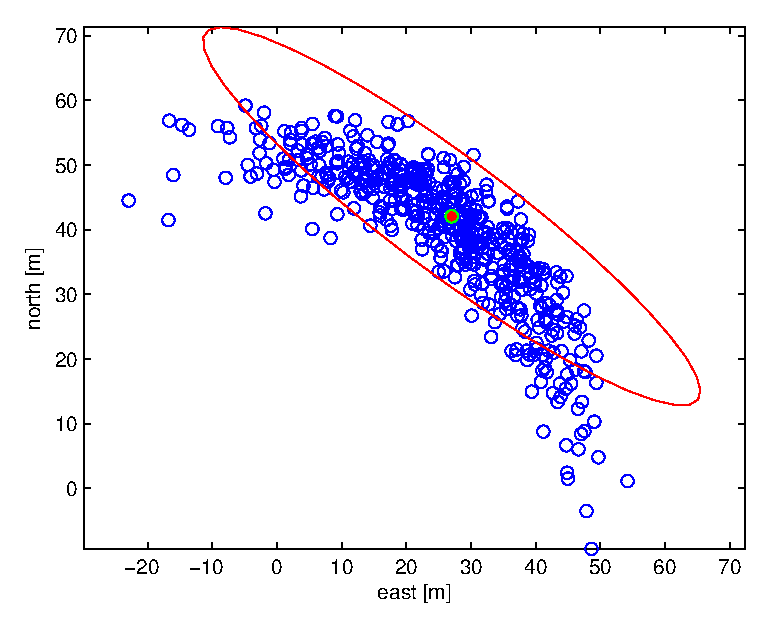
\includegraphics[width=0.40\textwidth]{kalman/fig/linear.eps}}      \\
    \subfigure[Original Gaussian random variable with samples selected by unscented transform algorithm.]
    {\label{fig:sigma-samples}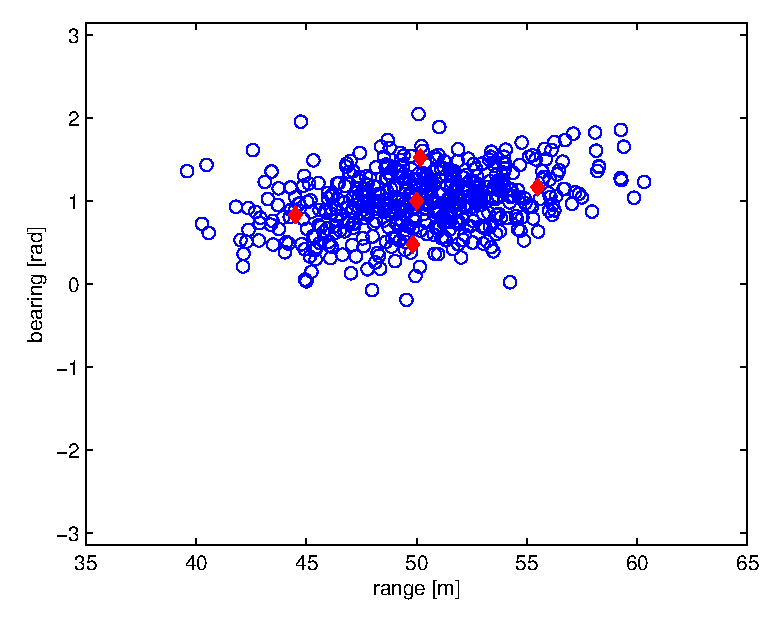
\includegraphics[width=0.40\textwidth]{kalman/fig/orig-samples.eps}}
    \subfigure[Gaussian variable after nonlinear transform with mean and variance (ellipse) estimated using unscented transform.]
    {\label{fig:unsc-transform}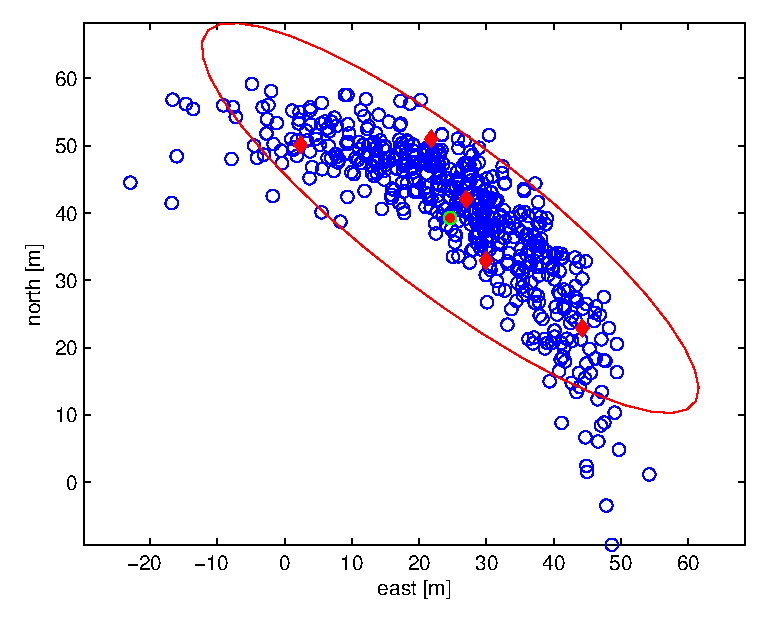
\includegraphics[width=0.40\textwidth]{kalman/fig/unscented.eps}}
  \end{center}
  \caption{Nonlinear transformation of a Gaussian random variable and estimation of its statistical parameters - mean and variance, using linearisation approximation and unscented transform.}
  \label{fig:gauss-transform}
\end{figure}

Calculation-wise, the whole procedure is fairly easier than linearisation algorithm since there is no need for calculating the Jacobian or Hessian, total number of computations stays the same and it is easier to improvise with the algorithm with constrains or parameters which define the way samples are selected. In addition, UT shown in example (Figure ~\ref{fig:gauss-transform} ) handles the whole distribution and its transformation by tracking only five samples. Higher dimensionality of GRV would result in more samples taken. However that number is still reasonably small compared with Monte Carlo methods.
\begin{algorithm}%[h!]
\caption{The Discrete Unscented Kalman Filter} \label{alg:ukf}
\begin{algorithmic}
\REQUIRE $\vect{\hat{x}}(0) = E\lbrace \vect{x}(0) \rbrace$
\COMMENT{initialize state}
\REQUIRE $\vect{P}(0) = \delta_{jk} \vect{P}_{0} $ 
\COMMENT {initialize covariance}
\REQUIRE $\vect{\hat{x}}^{aug}(0) = \left[ \begin{array}{c} \vect{\hat{x}}^{x}(0) \\ \vect{x}^{n}(0) \\ \vect{x}^{m}(0) \end{array} \right]
                                  = \left[ \begin{array}{c} \vect{\hat{x}}(0) \\ \vect{0} \\ \vect{0} \end{array} \right] $ 
\COMMENT{init. augmented state: state + process noise + meas. noise}
\STATE   $L = length(\vect{\hat{x}}^{aug}) \; k = const$
\COMMENT{augmented state length and $k$ parameter set}
\REQUIRE $\vect{P}^{aug}(0) = \left[ \begin{array}{ccc} \vect{P}_{0} & \vect{0}     & \vect{0} \\ 
															\vect{0} & \vect{P}_{n} & \vect{0} \\
															\vect{0} & \vect{0}     & \vect{P}_{m} \end{array} \right] $ 
\COMMENT{initialize augmented state covariance}
\LOOP
	\STATE $k \Leftarrow k+1$
	\STATE $\vect{A}^{aug}(k-1) = \left[\vect{\hat{x}}^{aug}(k-1) \vect{\hat{x}}^{aug}(k-1)\pm \sqrt{(L)\vect{P}^{aug}(k-1)}  \right] $
	\COMMENT {compute samples - unscented transform}
	\STATE   $ \vect{W}_{i}, \; i = 0,...,2L $
	\COMMENT {compute weights}
	\STATE   $\vect{A}^{x}(k \mid k-1) = f(vect{A}^{x}(k-1), vect{A}^{n}(k-1)) $
	\COMMENT {nonlinear process model}
	\STATE	 $ \vect{\hat{x}}(k \mid k-1) = \sum_{i=0}^{2L} \vect{W}_{i} \vect{A}^{x}_{i}(k \mid k-1) $
	\COMMENT {state prediction}
	\STATE   $ \vect{P}(k \mid k-1) = \sum_{i=0}^{2L} \vect{W}_{i} (\vect{A}^{x}_{i}(k \mid k-1) - \vect{\hat{x}}(k \mid k-1)) 
																   (\vect{A}^{x}_{i}(k \mid k-1) - \vect{\hat{x}}(k \mid k-1))^{T} $
	\COMMENT {state prediction uncertainty}
	\STATE   $\vect{Z}(k \mid k-1) = h(vect{A}^{x}(k-1), vect{A}^{m}(k-1)) $
	\COMMENT {nonlinear measurement model}
	\STATE   $\vect{\hat{Z}}(k) =  \sum_{i=0}^{2L} \vect{W}_{i} \vect{Z}_{i}(k \mid k-1)$
	\COMMENT {measurement prediction - unscented transform}
	\STATE   $\vect{P}_{zz} =  \sum_{i=0}^{2L} \vect{W}_{i} (\vect{Z}_{i}(k \mid k-1)-\vect{\hat{Z}}(k)) 
															(\vect{Z}_{i}(k \mid k-1)-\vect{\hat{Z}}(k))^{T}$
	\STATE   $\vect{P}_{xz} =  \sum_{i=0}^{2L} \vect{W}_{i} (\vect{A}_{i}(k \mid k-1)-\vect{\hat{x}}(k \mid k-1))
															(\vect{Z}_{i}(k \mid k-1)-\vect{\hat{Z}}(k))^{T}$
	\STATE   $\vect{K}      = \vect{P}_{xz} \vect{P}_{zz}^{-1}$
	\STATE	 $ \vect{\hat{x}}(k) = \vect{\hat{x}}(k \mid k-1) + \vect{K} (\vect{z}(k) - \vect{\hat{Z}}(k))  $
	\COMMENT {state correction}
	\STATE   $ \vect{P}(k) = \vect{P}(k \mid k-1) - \vect{K} \vect{P}_{zz} \vect{K}^{T} $
	\COMMENT {state correction uncertainty}	
	\RETURN $\vect{\hat{x}}(k), \vect{P}(k)$
\ENDLOOP
\end{algorithmic}
\end{algorithm}